% Better comment extension for Vscode colors these comments differently
% Normal comment color
% * Important information
% ! ALERT
% ? Question
% TODO stuff to do
% // This is strikethrough



MY NOTEPAD, this is not imported anywhere


% ! NEW code
\begin{tikzpicture}[scale=0.5]
    % Define the tiles
    \def\tileA{(0,0) rectangle (1,1)}
    \def\tileB{(1,0) rectangle (2,1)}
    
    % Draw the tiling pattern
    \foreach \x in {0,1,2,3}{
      \foreach \y in {0,1}{
        \draw \tileA (\x,\y);
        \draw \tileB (\x+0.5,\y+0.5);
      }
    }
  \end{tikzpicture}


% ! NEW code
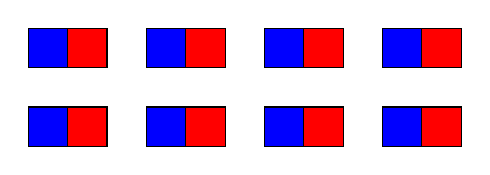
\begin{tikzpicture}[scale=0.5]
    % Define the tile
    \def\tile{
      % Insert TikZ commands for the tile here
      \draw[fill=blue] (0,0) rectangle (1,1);
      \draw[fill=red] (1,0) rectangle (2,1);
    }
    
    % Draw the tiling pattern
    \foreach \x in {0,1,2,3}{
      \foreach \y in {0,1}{
        \pgfmathsetmacro{\shiftX}{\x*3} % Set horizontal shift
        \pgfmathsetmacro{\shiftY}{\y*2} % Set vertical shift
        \begin{scope}[shift={(\shiftX,\shiftY)}]
          \tile
        \end{scope}
      }
    }
  \end{tikzpicture}

% ! NEW code
  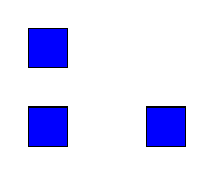
\begin{tikzpicture}[scale=0.5]
    % Define the tile
    \def\tile{
      % Insert TikZ commands for the tile here
      \draw[fill=blue] (0,0) rectangle (1,1);
      %\draw[fill=red] (1,0) rectangle (2,1);
    }
    
    % Draw the tiling pattern
    \tile % Draw the first tile at the origin
    \begin{scope}[shift={(3,0)}]
      \tile % Draw the second tile shifted three units to the right
    \end{scope}
    \begin{scope}[shift={(0,2)}]
      \tile % Draw the third tile shifted two units up
    \end{scope}
    % Continue adding more tiles with different shift values to create the desired tiling pattern
  \end{tikzpicture}


% ! NEW code
  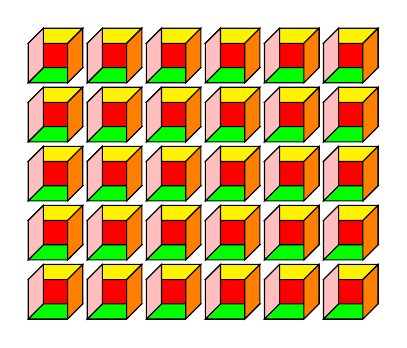
\begin{tikzpicture}[scale=0.5]
    % Define the tile
    \def\tile{
      % Draw the unit cube
      \draw[fill=blue] (0,0,0) -- (1,0,0) -- (1,1,0) -- (0,1,0) -- cycle;
      \draw[fill=red] (0,0,1) -- (1,0,1) -- (1,1,1) -- (0,1,1) -- cycle;
      \draw[fill=green] (0,0,0) -- (1,0,0) -- (1,0,1) -- (0,0,1) -- cycle;
      \draw[fill=yellow] (0,1,0) -- (1,1,0) -- (1,1,1) -- (0,1,1) -- cycle;
      \draw[fill=pink] (0,0,0) -- (0,1,0) -- (0,1,1) -- (0,0,1) -- cycle;
      \draw[fill=orange] (1,0,0) -- (1,1,0) -- (1,1,1) -- (1,0,1) -- cycle;
    }
  
    % Draw the tiling pattern
    \foreach \x in {0,1,2,3,4,5}{
      \foreach \y in {0,1,2,3,4}{
        \pgfmathsetmacro{\shiftX}{\x*1.5} % Set horizontal shift
        \pgfmathsetmacro{\shiftY}{\y*1.5} % Set vertical shift
        \begin{scope}[shift={(\shiftX,\shiftY,0)}]
          \tile % Draw the tile
        \end{scope}
      }
    }
  \end{tikzpicture}

  % ! NEW code
  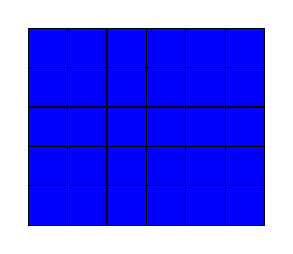
\begin{tikzpicture}[scale=0.5]
    % Define the tile
    \def\tile{
      % Draw the unit square with fill color
      \draw[fill=blue] (0,0) rectangle (1,1);
    }
  
    % Draw the tiling pattern
    \foreach \x in {0,1,2,3,4,5}{
      \foreach \y in {0,1,2,3,4}{
        \pgfmathsetmacro{\shiftX}{\x} % Set horizontal shift
        \pgfmathsetmacro{\shiftY}{\y} % Set vertical shift
        \begin{scope}[shift={(\shiftX,\shiftY)}]
          \tile % Draw the tile
        \end{scope}
      }
    }
  \end{tikzpicture}

% ! NEW code
  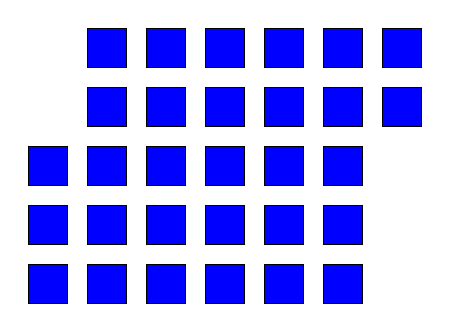
\begin{tikzpicture}[scale=0.5]
    % Define the tile
    \def\tile{
      % Draw the unit square with fill color
      \draw[fill=blue] (0,0) rectangle (1,1);
    }
  
    % Draw the tiling pattern
    \foreach \x in {0,1,2,3,4,5}{
      \foreach \y in {0,1,2,3,4}{
        \pgfmathsetmacro{\shiftX}{\x*1.5 + (1.5*\y > 3.5 ? 1.5 : 0)} % Set horizontal shift
        \pgfmathsetmacro{\shiftY}{\y*1.5} % Set vertical shift
        \begin{scope}[shift={(\shiftX,\shiftY)}]
          \tile % Draw the tile
        \end{scope}
      }
    }
  \end{tikzpicture}



  % ! NEW code
  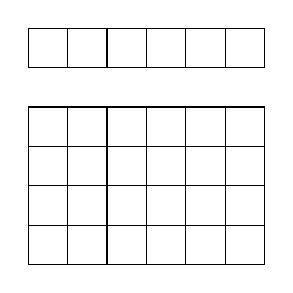
\begin{tikzpicture}[scale=0.5]
    % Define the tile
    \def\tile{
      % Draw the unit square
      \draw (0,0) rectangle (1,1);
    }
  
    % Draw the tiling pattern
    \foreach \x in {0,1,2,3,4,5}{
      \foreach \y in {0,1,2,3,4}{
        \pgfmathsetmacro{\shiftX}{\x} % Set horizontal shift
        \pgfmathsetmacro{\shiftY}{\y + (\y > 3.5 ? 1:0)} % Set vertical shift
        \begin{scope}[shift={(\shiftX,\shiftY)}]
          \tile % Draw the tile
        \end{scope}
      }
    }
  \end{tikzpicture}

% ! NEW code
  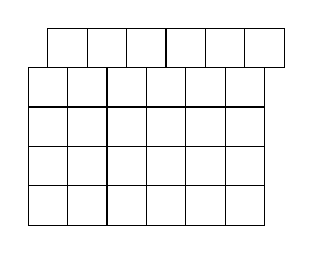
\begin{tikzpicture}[scale=0.5]
    % Define the tile
    \def\tile{
      % Draw the unit square
      \draw (0,0) rectangle (1,1);
    }
  
    % Draw the tiling pattern
    \foreach \x in {0,1,2,3,4,5}{
      \foreach \y in {0,1,2,3,4}{
        \pgfmathsetmacro{\shiftX}{\x + (\y > 3.5 ? 0.5 : 0)} % Set horizontal shift
        \pgfmathsetmacro{\shiftY}{\y} % Set vertical shift
        \begin{scope}[shift={(\shiftX,\shiftY)}]
          \tile % Draw the tile
        \end{scope}
      }
    }
  \end{tikzpicture}


% ! NEW code
  
\begin{tikzpicture}[scale=0.5]
    % Define the tile
    \def\tile{
      % Draw the unit square
      \draw (0,0) rectangle (1,1);
    }
  
    % Draw the tiling pattern
    \foreach \x in {0,1,2,3,4,5}{
      \foreach \y in {0,1,2,3,4}{
        \pgfmathsetmacro{\shiftX}{\x} % Set horizontal shift
        \pgfmathsetmacro{\shiftY}{\y + (3.5 > \x > 2.5 ? 0.5 : 0)} % Set vertical shift
        \begin{scope}[shift={(\shiftX,\shiftY)}]
          \tile % Draw the tile
        \end{scope}
      }
    }
  \end{tikzpicture}

% ! NEW code
  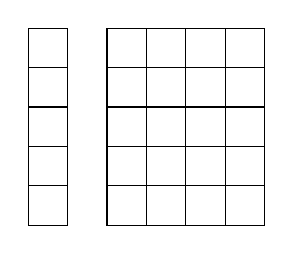
\begin{tikzpicture}[scale=0.5]
    % Define the tile
    \def\tile{
      % Draw the unit square
      \draw (0,0) rectangle (1,1);
    }
  
    % Draw the tiling pattern
    \foreach \x in {0,1,2,3,4,5}{
      \ifnum\x < 3
        \pgfmathsetmacro{\shiftX}{\x + (\x > 0 ? 1 : 0)} % Set horizontal shift
      \else
        \pgfmathsetmacro{\shiftX}{\x} % No horizontal shift for the last three columns
      \fi
      \foreach \y in {0,1,2,3,4}{
        \pgfmathsetmacro{\shiftY}{\y} % No vertical shift
        \begin{scope}[shift={(\shiftX,\shiftY)}]
          \tile % Draw the tile
        \end{scope}
      }
    }
  \end{tikzpicture}

% ! NEW code
  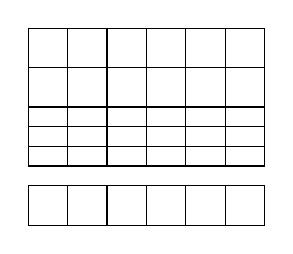
\begin{tikzpicture}[scale=0.5]
    % Define the tile
    \def\tile{
      % Draw the unit square
      \draw (0,0) rectangle (1,1);
    }
  
    % Draw the tiling pattern
    \foreach \x in {0,1,2,3,4,5}{
      \foreach \y in {0,1,2,3,4}{
        \pgfmathsetmacro{\shiftX}{\x} % No horizontal shift
        \ifnum\y<2
          \pgfmathsetmacro{\shiftY}{\y + (\y > 0 ? 0.5 : 0)} % Set vertical shift
        \else
          \pgfmathsetmacro{\shiftY}{\y} % No vertical shift for the last three rows
        \fi
        \begin{scope}[shift={(\shiftX,\shiftY)}]
          \tile % Draw the tile
        \end{scope}
      }
    }
  \end{tikzpicture}


% ! NEW code
  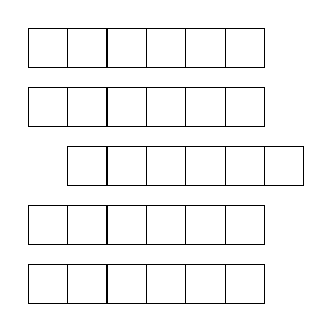
\begin{tikzpicture}[scale=0.5]
    % Define the tile
    \def\tile{
      % Draw the unit square
      \draw (0,0) rectangle (1,1);
    }
  
    % Draw the tiling pattern
    \foreach \x in {0,1,2,3,4,5}{
      \foreach \y in {0,1,2,3,4}{
        \ifnum\y=2 % Set horizontal shift for the third row only
          \pgfmathsetmacro{\shiftX}{\x + 1} % Shift one unit to the right
        \else
          \pgfmathsetmacro{\shiftX}{\x} % No horizontal shift for other rows
        \fi
        \pgfmathsetmacro{\shiftY}{\y} % No vertical shift
        \begin{scope}[shift={(\shiftX,\shiftY*1.5)}]
          \tile % Draw the tile
        \end{scope}
      }
    }
  \end{tikzpicture}






%* 
Til bruk for plotsene
When representing this in a figure, one should note the similarity to a cross product of spaces such as $\Z \times \Z$ or $\R \times \R$. Most important in the construction of spectra presented \cref{thrm:construction_spectra} is that it opens up the possibility of having a different discrete set at each $\lambda_1$-value. This newfound flexibility will be discussed after the proof of the \namecref{thrm:construction_spectra}.
%? VURDERE. Før "When representing" ha: Note that we would still have that the zero-element is the only element that is orthogonal to both sets.



% * In \cite{jorgensenSpectralPairsCartesian2001} Steen P. and Palle E. presented a method on the construction of spectral pairs in higher dimensions. It is a recursive technique in what they dub "a cross-product construction" using "factors" in lower dimensions and applies for any two spectral pairs $\brac{\Omega_i,\Lambda_i}$ where $i=1,2$ and in arbitrary dimensions $d_1$ and $d_2$. The technique is presented in the following theorem



%* Second construction
\begin{example}\label{exmp:second_construction}
    Let $\brac{\Omega_1,\Lambda_1} = \brac{I^2, \Lambda}$, where $\Lambda$ is as given in \labelcref{eq:first_construction}. If we again let 
    $\brac{\Omega_2,\Lambda(\lambda_1)} = \brac{I, \Z}$ for all $\lambda_1 \in \Lambda_1$ as in the previous \namecref{exmp:first_construction}, it then also follows from \cref{thrm:construction_spectra} that $\brac{I^2 \times I, \Lambda'}$ is a spectral pair in $2+1=3$ dimensions where 
    \begin{equation*}
        \Lambda'=\braq{\brac{\lambda_1,\lambda_2}: \lambda_1 \in \Lambda, \lambda_2 \in \Z }.
    \end{equation*}
    Similarly, we can also show that $\brac{I^2 \times I^2, \Lambda''}$ is a spectral pair in $2+2=4$ dimensions with
    \begin{equation*}
        \Lambda''=\braq{\brac{\lambda_1,\lambda_2}: \lambda_1 \in \Lambda, \lambda_2 \in \Lambda} \qedhere
    \end{equation*}
\end{example}




% We consider orthogonal sets with a focus on countable orthogonal sequences. 
Let $H$ be a hilbert space, and $\left\{ e_{n} \right\}_{n\in \mathbb{N}}$ denote a sequence of orthonormal vectors in $H$. Then the closed span, $\overline{\operatorname{span}}\left( \left\{ e_{n} \right\}_{n\in \mathbb{N}} \right)$, is a closed subspace of $H$. In connection with this, we can give an explicit formula for the orthogonal projection of a vector onto $\overline{\operatorname{span}}\left( \left\{ e_{n} \right\}_{n\in \mathbb{N}} \right)$. This is presented in the following theorem \cite[p.~210]{heilMetricsNormsInner2018}.
%
%
\begin{theorem}\label{thrm:orthog_proj_formula_and_facts}
    If $H$ is a Hilbert space and if $\left\{ e_{n} \right\}_{n\in \mathbb{N}}$ is an orthonormal sequence in $H$,  then the following statements hold:
    \begin{enumerate}[label=(\alph*)]
        \item \label{eq:opfaf_a} Bessel's inequality holds for all $x \in H$. That is, 
        \begin{equation}
            \sum_{n=1}^{\infty} \left| \langle x, e_n \rangle \right|^2 \leq \| x\|^2 
        \end{equation}
        
        \item \label{eq:opfaf:b} Let $c_n$ be scalars. If the series $$ x=\sum_{n=1}^\infty c_n e_n.$$ converges in the norm of $H$, then the scalars $c_n= \langle x, e_n\rangle$ for each $n \in \mathbb{N}$.
        
        \item \label{eq:opfaf_c} The following equivalence: 
        \begin{equation}
            \sum_{n=1}^{\infty} c_n e_n \text{ converges in norm of } H \Longleftrightarrow \sum_{n=1}^{\infty} \left| c_n \right|^2 < \infty.
        \end{equation}
        In this case the series $\sum_{n=1}^{\infty} c_n e_n$ converges unconditionally, meaning that it converges regardless of the ordering of the index set.
        
        \item \label{eq:opfaf_d} If $x \in H$, then 
        \begin{equation} 
            p= \sum_{n=1}^{\infty} \langle x, e_n \rangle e_n, 
        \end{equation} 
        is the orthogonal projection of $x$ onto  $\overline{\operatorname{span}} \left( \left\{ e_{n} \right\}_{n\in \mathbb{N}} \right) $, with
        \begin{equation}
            \| p\|^2 = \sum_{n=1}^{\infty} \left| \langle x,e_n \rangle \right|^2
        \end{equation}
        
        \item \label{eq:opfaf_e} If $x \in H$, then 
        \begin{equation}
            x\in \overline{\operatorname{span}} \left( \left\{ e_{n} \right\}_{n\in \mathbb{N}} \right) \Longleftrightarrow x=\sum_{n=1}^{\infty} \langle x, e_n \rangle e_n \Longleftrightarrow \| x\|^2 = \sum_{n=1}^{\infty} \left| \langle x,e_n\rangle \right|^2
        \end{equation}
    \end{enumerate}
\end{theorem}
%
%
% ! Max Kommentar
\textcolor{red}{poof}\\
Intro, ONB
%
%
\begin{theorem}\label{thrm:orthonormal_equivalences}
    If $H$ is a Hilbert space and if $\left\{ e_{n} \right\}_{n\in \mathbb{N}}$ is an orthonormal sequence in $H$,  then the following are equivalent:
    \begin{enumerate}[label=(\alph*)]
        \item \label{eq:oe_a} $\left\{ e_{n} \right\}_{n\in \mathbb{N}}$ is complete. That is, $\overline{\operatorname{span}} \left( \left\{ e_{n} \right\}_{n\in \mathbb{N}} \right) = H$
        
        \item \label{eq:oe_b} $\left\{ e_{n} \right\}_{n\in \mathbb{N}}$ is a \emph{Schauder basis} for $H$. That is, for each $x\in H$ there exists a unique sequence  $(c_n)_{n\in\mathbb{N}}$ of scalars such that $x = \sum c_n x_n$.
        
        \item \label{eq:oe_c} If $x\in H$, then the following series converges in the norm of $H$. \begin{equation} \label{eq:orthonormal_equivalences_3} x=\sum_{n=1}^\infty \langle x,e_n\rangle e_n, \end{equation}
        
        \item \label{eq:oe_d} Plancherel's equality holds for all $x \in H$. That is, $$ \|x \|^2 = \sum_{n=1}^\infty \left| \langle x,e_n \rangle \right|^2.$$
        
        \item \label{eq:oe_e} Parseval's equality holds for all $x,y \in H$. That is, $$ \langle x,y \rangle = \sum_{n=1}^\infty \langle x,e_n \rangle \langle e_n,y \rangle $$
    \end{enumerate}
\end{theorem}

Note that a sequence that satisfies any of the equivalent conditions in \cref{thrm:orthonormal_equivalences} is an orthonormal basis. We form the following definition.




\begin{definition}\label{def:ONB}
    A countable infinite orthonormal sequence $\left\{ e_{n} \right\}_{n\in \mathbb{N}}$ that is complete in a Hilbert space $H$ is called an \emph{orthonormal basis} for $H$.
\end{definition}

\begin{definition}\label{def:ONB}
    Let $H$ be a Hilbert space. A countable infinite orthonormal sequence $\left\{ e_{n} \right\}_{n\in \mathbb{N}}$ that is complete in a Hilbert space $H$ is called an \emph{orthonormal basis} for $H$.
\end{definition}




